\documentclass[spanish]{article}                 % Tipo de documento
\usepackage[left=1in,right=1in,top=1in,          % Márgenes
            bottom=1in,footskip=0.5in]{geometry}
\usepackage[T1]{fontenc}                         % Codificación
\usepackage[utf8]{inputenc}
\usepackage[spanish, activeacute]{babel}         % Idioma español
\usepackage{newtxtext}
\usepackage{charter} % Fuente
\decimalpoint{}

\usepackage{amsmath, amsthm, amssymb}            % Entornos y símbolos ams
\numberwithin{equation}{section}                 % Numeración de ecuaciones
\newtheorem{teorema}{Teorema}[section]           % Teoremas y su numeración
\newtheorem{corolario}[teorema]{Corolario}
\newtheorem{lema}[teorema]{Lema}
\newtheorem{proposición}[teorema]{Proposición}
\theoremstyle{definition}
\newtheorem{definición}[teorema]{Definición}
\newtheorem{problema}{Problema}[section]
\newtheorem{solución}{Solución}

\usepackage{graphicx}                            % Usar imágenes
\usepackage{subfigure}
\usepackage[italic]{esdiff}                      % Derivadas
\usepackage{mathtools}

\usepackage{dsfont}
                                                      % Operadores
\DeclarePairedDelimiter\abs{\lvert}{\rvert}           % Valor absoluto
\DeclarePairedDelimiter\norm{\lVert}{\rVert}          % Normas
\newcommand{\argmin}{\mathop{\mathrm{argmin}}\limits} % ArgMin
\newcommand{\argmax}{\mathop{\mathrm{argmax}}\limits} % ArgMax
\newcommand*\dif{\mathop{}\!\mathrm{d}}               % Diferencial para integrales

\DeclareMathOperator{\Sim}{sim} % Similarity
\DeclareMathOperator{\RMSE}{RMSE}
\DeclareMathOperator{\MAE}{MAE}

\title{Sistemas de recomendación}
\author{Eduardo Alexis Romo Almazán}
% \date{}

%%%%%%%%%%%%%%%%%%%%%%%%%%%%%%%%%%%%%%%%%%%%%%%%%%%%%%%%%%%%%%%%%%%%%%%
%                              Documento                              %
%%%%%%%%%%%%%%%%%%%%%%%%%%%%%%%%%%%%%%%%%%%%%%%%%%%%%%%%%%%%%%%%%%%%%%%
\begin{document}
\maketitle

\section{Métodos basados en promedios}~\label{sec:basados_en_promedios}
Este método toma el promedio de los valores conocidos y los utiliza para predecir las entradas de $M$. Se pueden hacer 3 variantes:
\begin{itemize}
    \item Tomar el promedio de todos los valores conocidos y predecir $\hat M_{i, j} = \bar M$ para todo $i$ y todo $j$.
    \item Tomar el promedio de valores conocidos por filas y predecir $\hat M_{i, j} = \bar M_i$ para todo $i$ y todo $j$.
    \item Tomar el promedio de valores conocidos por columnas y predecir $\hat M_{i, j} = \bar M_{:,j}$ para todo $i$ y todo $j$.
\end{itemize}

\section{Métodos basados en similitud de filas o columnas}
\subsection{Basado en filas}
Para predecir el valor de la entrada $(i, j)$ de la matriz, se obtiene una lista de las $r$ filas más parecidas a la fila $i$ y tomamos un promedio pesado de los valores $(k, j)$ de la siguiente manera:

\begin{equation}
    \label{eq:row_based}
    \hat M_{i, j} = \frac{\sum_{k \in W(i)}\Sim(i, k) M_{k, j}}{\sum_{k \in W(i)} \Sim(i, k)},
\end{equation}
donde $W(i)$ es el conjunto de las $r$ filas más parecidas a $M_i$.

\subsection{Basado en columnas}

De manera análoga a la predicción basada en filas, se encuentran las $r$ columnas más parecidas a $M_{:,j}$ para predecir $M_{i, j}$
\begin{equation}
    \label{eq:col_based}
    \hat M_{i, j} = \frac{\sum_{k \in W(j)}\Sim(j, k) M_{i, k}}{\sum_{k \in W(j)} \Sim(j, k)},
\end{equation}
donde $W(j)$ es el conjunto de las $k$ columnas más parecidos a $M_{:,j}$.

\subsection{Medidas de similitud}~\label{sec:medidas_similitud}
En las ecuaciones~\ref{eq:row_based}~y~\ref{eq:col_based} es necesaria una función de similitud entre filas o columnas. Algunas de las medidas usadas son las siguientes

\begin{itemize}
    \item Coeficiente de correlación de Pearson
        \begin{equation*}
            \Sim(x, y) = \frac{\sum_{i}^{}\left(x_i - \bar x \right) \left(y_i - \bar y \right)}{\sqrt{\sum_{i}^{} \left(x_i - \bar x\right)^2}\sqrt{\sum_{i}^{} \left(y_i - \bar y \right)^2}}
        \end{equation*}
    \item Similitud coseno
        \begin{equation*}
            \Sim(x, y) = \frac{x \cdot y}{\norm{x}_2 \norm{y}_2}
        \end{equation*}
    \item Mean absolute difference (*)
        \begin{equation*}
            \Sim(x, y) = \frac{1}{n}\sum_{i}^{} \abs{x_i - y_i}
        \end{equation*}
    \item Mean squared difference (*)
        \begin{equation*}
            \Sim(x, y) = \frac{1}{n}\sum_{i}^{} (x_i - y_i)^2
        \end{equation*}
\end{itemize}
    
Para utilizar estas medidas en las ecuaciones antes mencionadas, se toman los vectores que contienen únicamente los valores que son conocidos en ambas filas o en ambas columnas.

En las medidas marcadas con (*) se utiliza la siguiente transformación para tomar valores únicamente en el intervalo $[0, 1]$.
\begin{equation*}
    f(x) = \frac{2}{1 + \exp(x)}
\end{equation*}

\section{Bases de datos}

\subsection{Conjuntos de entrenamiento y pruebas}
Los valores conocidos de la matriz $M$ se dividen en dos subconjuntos: de entrenamiento y de prueba. El conjunto de entrenamiento se utiliza para predecir los valores que no se conocen, mientras que el conjunto de prueba se utiliza para evaluar el desempeño de cada método.

Usualmente se utilizará un $80\%$ de los datos conocidos en el conjunto de entrenamiento y un $20\%$ en el conjunto de prueba. Estos dos conjuntos no necesariamente van a ser disjuntos.

\subsection{Netflix\_3m1k}
Esta será la principal base de datos con la que vamos a hacer pruebas. Consiste en 4427 usuarios, 1000 items y 56136 clasificaciones, es decir, una densidad del 1.27 \%. Las clasificaciones están distribuidas como se muestra en la figura~\ref{fig:netflix_data_distribution}. Podemos observar que la mayoría de las clasificaciones son 3, 4, o 5. De lo anterior, podríamos interpretar que las personas solo califican las películas que sí les gustaron, en otro caso prefieren no dar una calificación en lugar de dar una muy baja.

Luego, en las figuras~\ref{fig:means_and_vars_by_row}~y~\ref{fig:means_and_vars_by_col} se observan las distribuciones de medias y varianzas por filas y columnas, respectivamente. Notemos que tanto en filas como columnas hay picos en los números enteros y muchas varianzas con valor cero. Con eso podemos decir que muchas de las personas siempre dieron la misma calificación a todas las películas que han visto.

% \begin{table}[h]
%     \centering
%     \caption{Bases de datos}
%     \begin{tabular}{|l|c|c|c|c|}
%         \hline
%         Base de datos & Usuarios & Items & Clasificaciones & Densidad \\ \hline 
%         Netflix3m1k & 4427 & 1000 & 56136 & 1.27 \% \\\hline
%     \end{tabular}
% \end{table}

\begin{figure}[ht]
    \centering
    \includegraphics[width=0.4\linewidth]{../Results/Netflix/Plots/Data_distribution.png}
    \caption{Distribución de clasificaciones en Netflix\_3m1k}\label{fig:netflix_data_distribution}
\end{figure}

\begin{figure}[ht]
    \centering
    \subfigure[Medias]{\includegraphics[width=0.4\linewidth]{../Results/Netflix/Plots/Hist_Mean_Rows.png}}
    \subfigure[Varianzas]{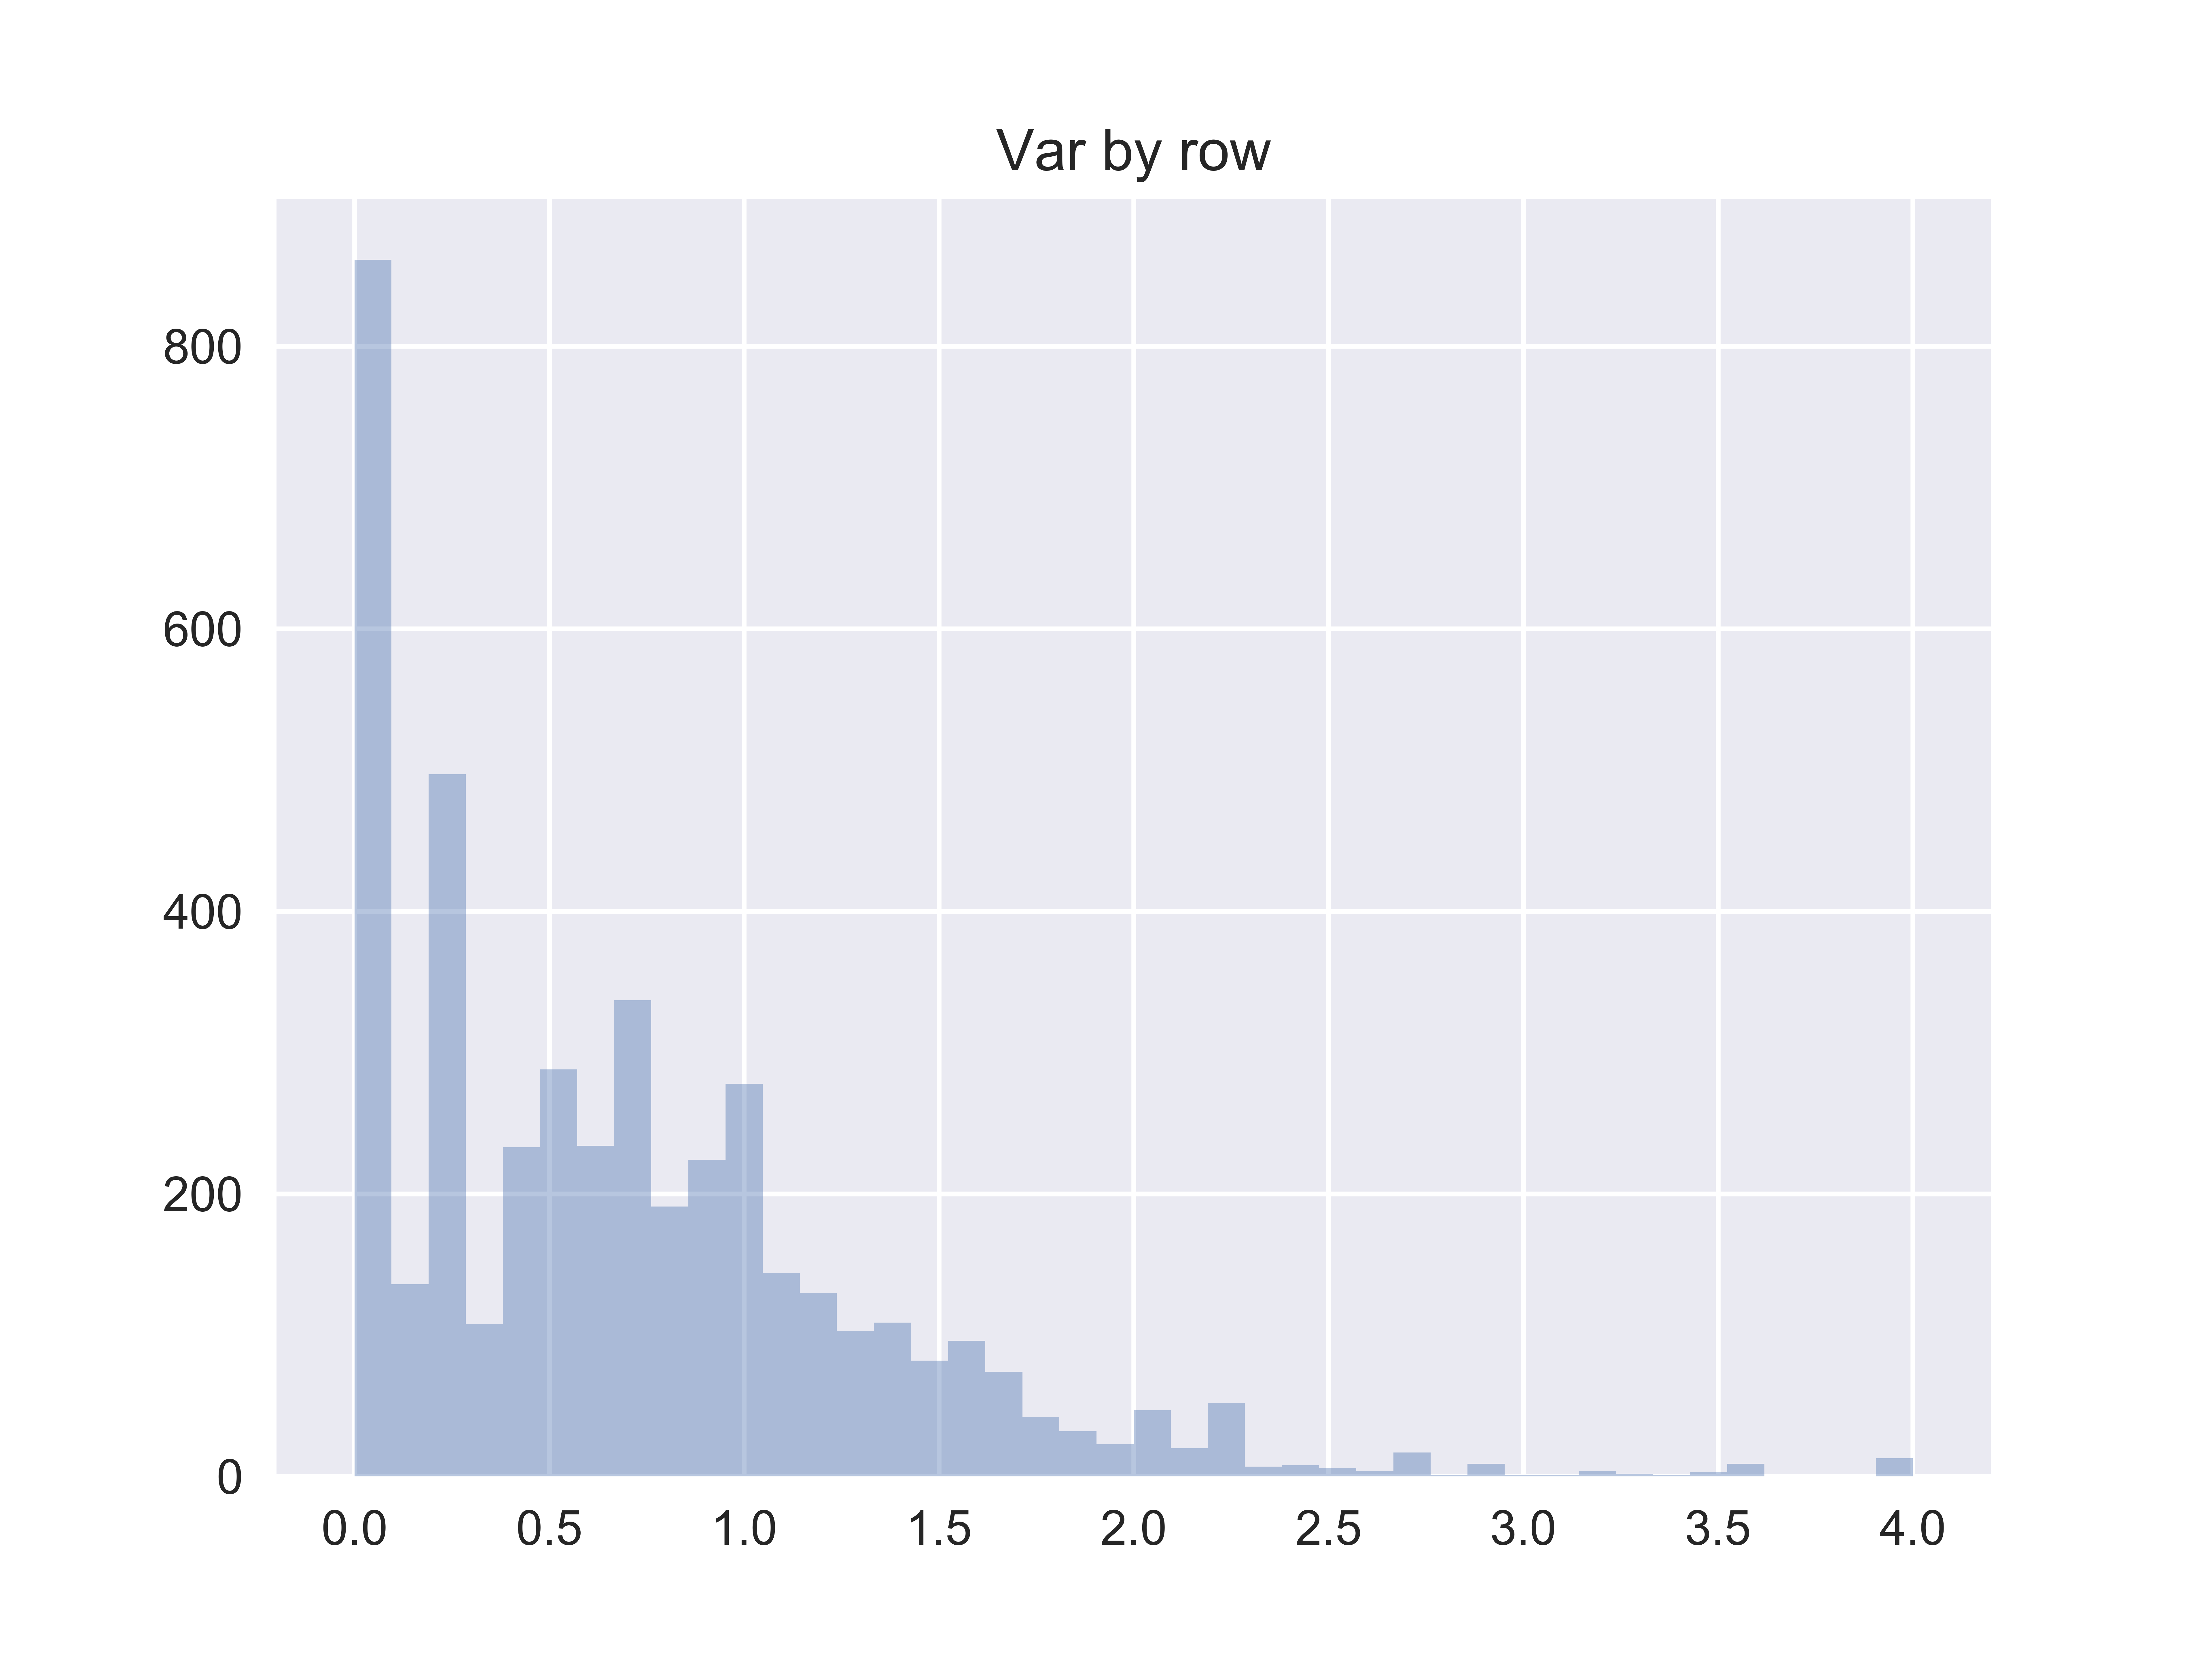
\includegraphics[width=0.4\linewidth]{../Results/Netflix/Plots/Hist_Var_Rows.png}}
    \caption{Medias y varianzas por filas}\label{fig:means_and_vars_by_row}
\end{figure}

\begin{figure}[ht]
    \centering
    \subfigure[Medias]{\includegraphics[width=0.4\linewidth]{../Results/Netflix/Plots/Hist_Mean_Cols.png}}
    \subfigure[Varianzas]{\includegraphics[width=0.4\linewidth]{../Results/Netflix/Plots/Hist_Var_Cols.png}}
    \caption{Medias y varianzas por columnas}\label{fig:means_and_vars_by_col}
\end{figure}

% \begin{figure}[htb]
%     \centering
%     \subfigure[Por número de vecinos]{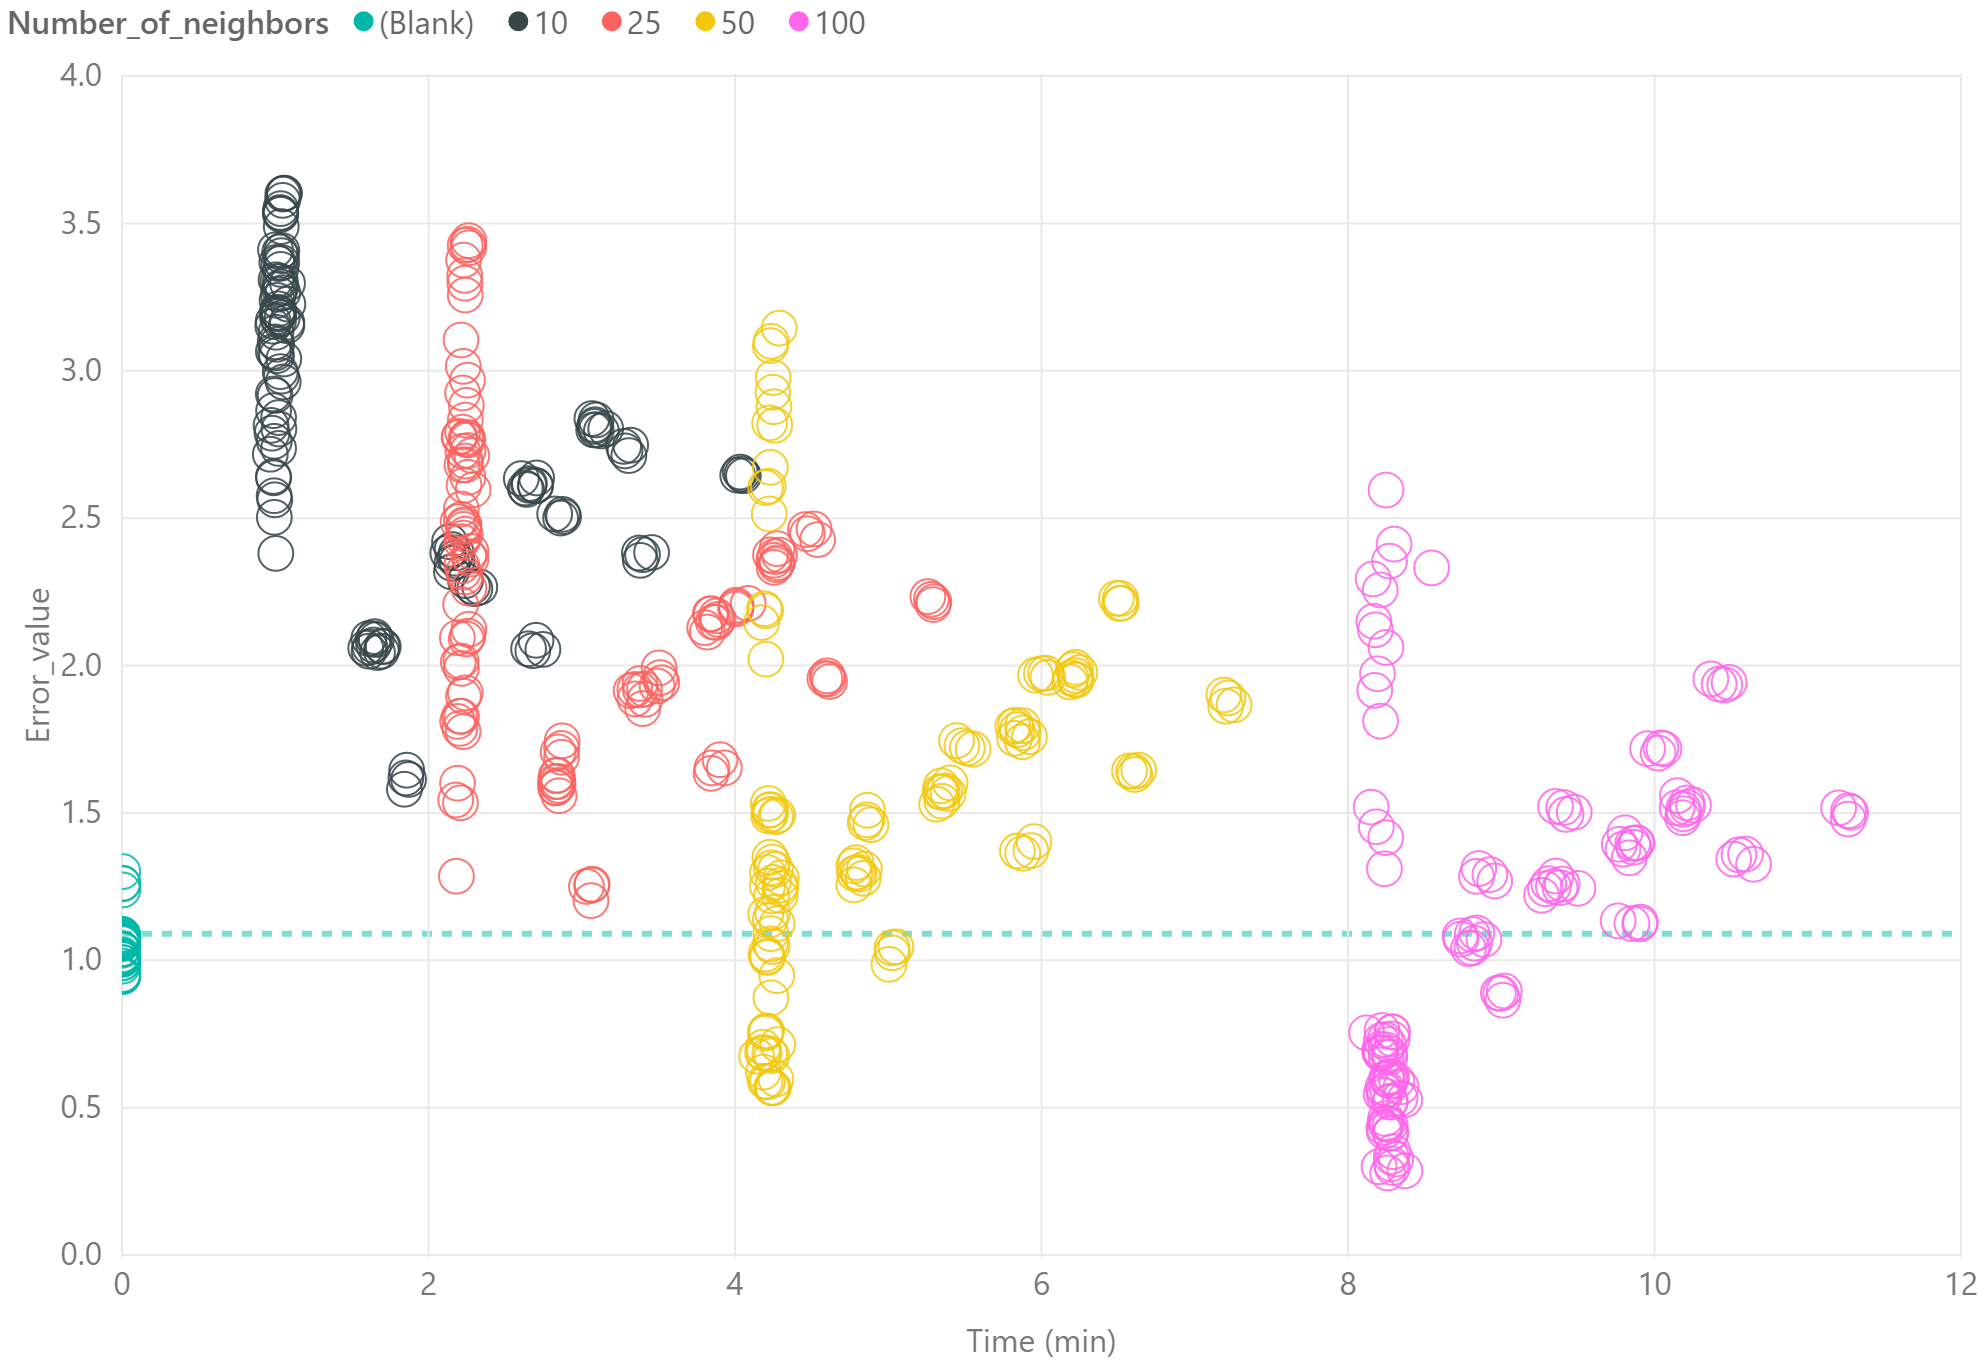
\includegraphics[width=0.60\linewidth]{../Results/Netflix/Plots/Time_RMSE_by_Neighbors.PNG}}
%     \subfigure[Por medida de similitud]{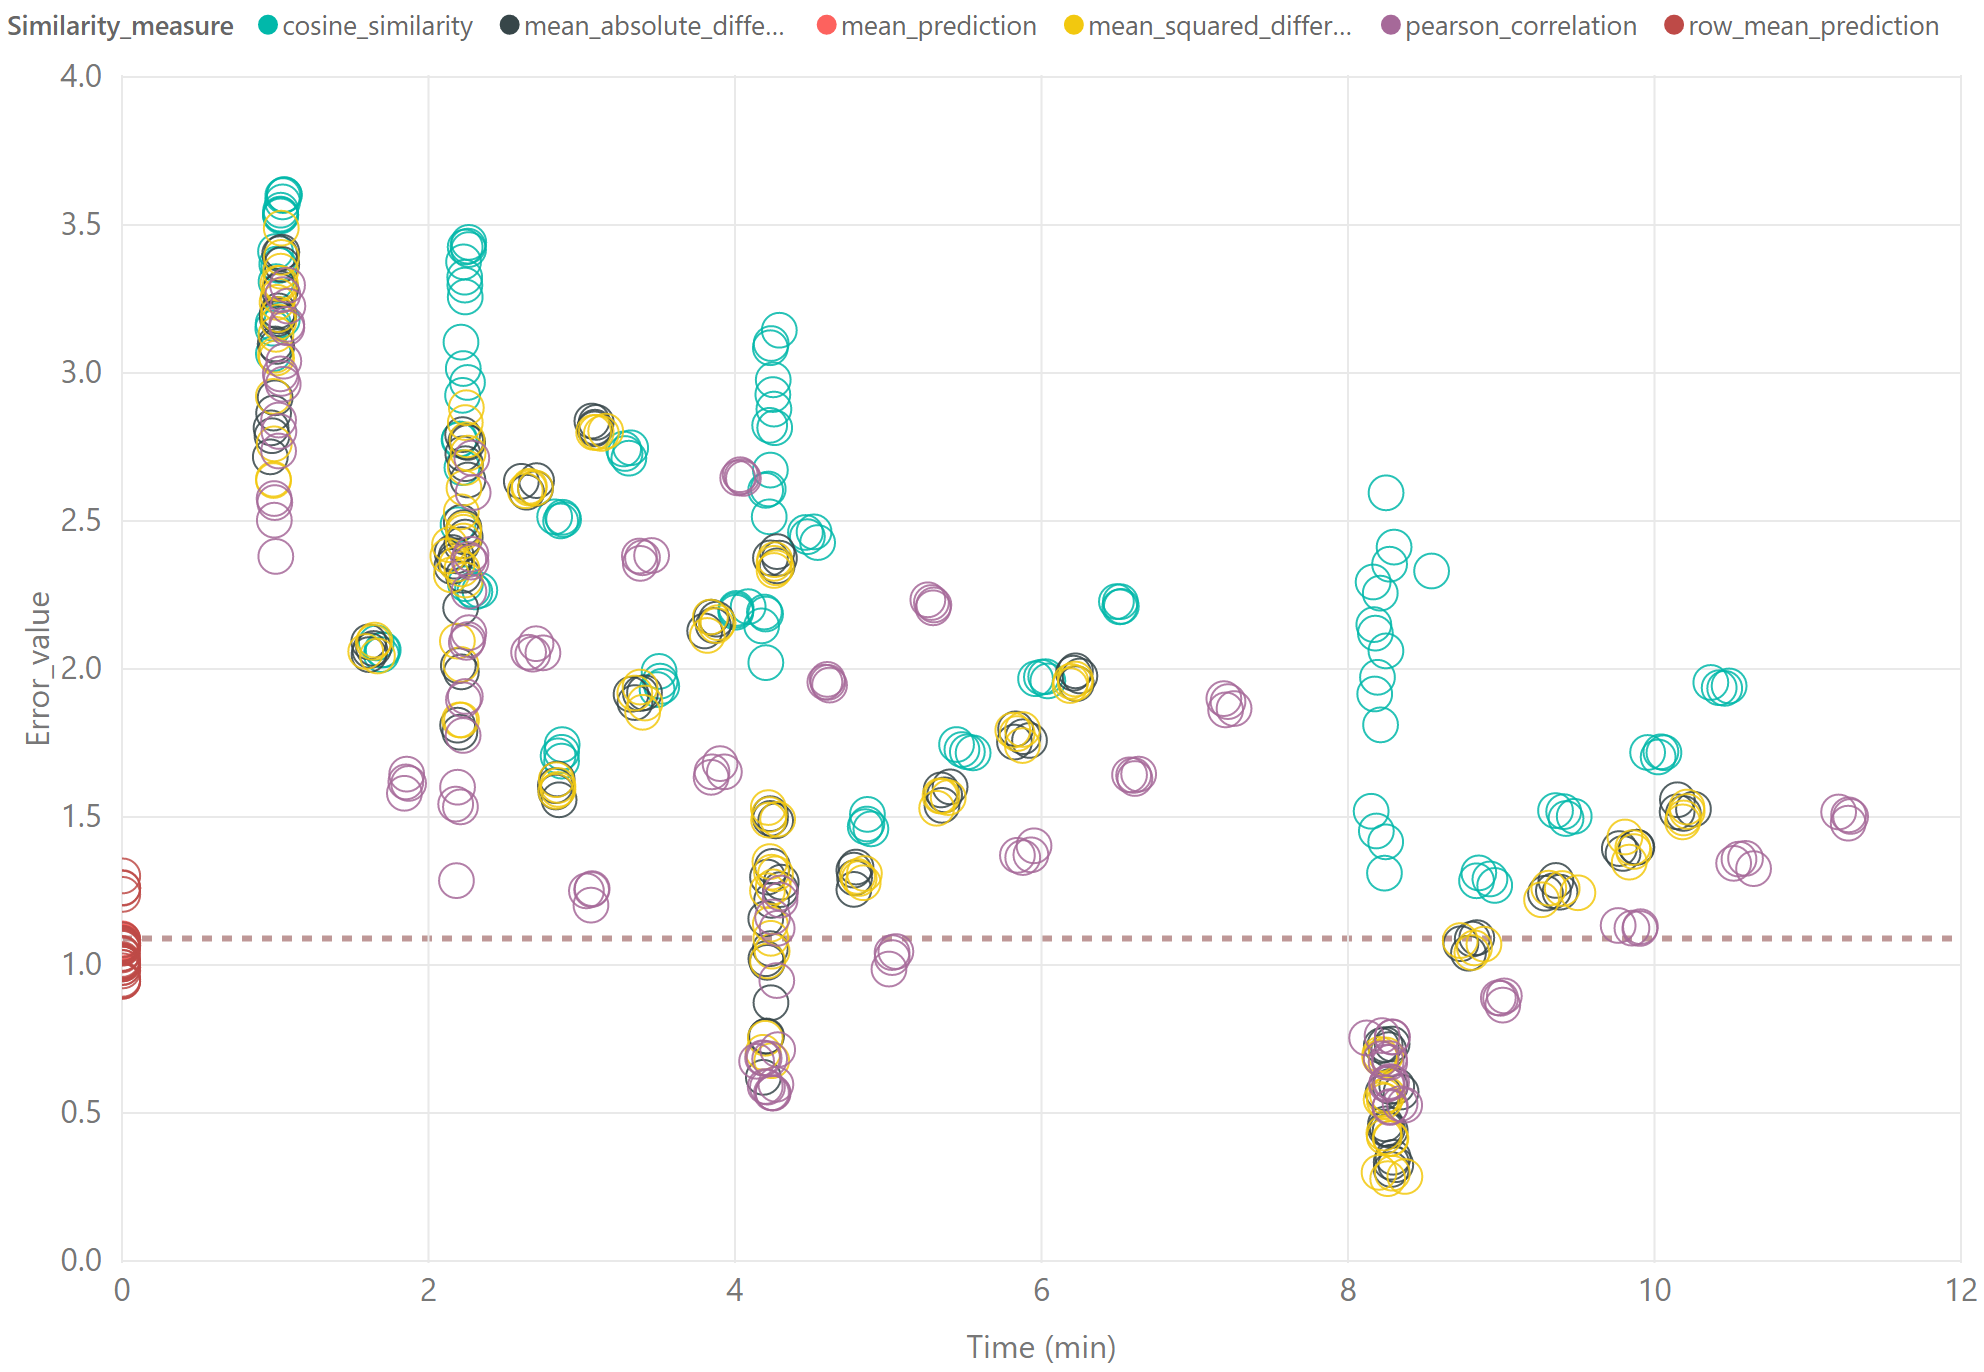
\includegraphics[width=0.60\linewidth]{../Results/Netflix/Plots/Time_RMSE_by_Similarity.PNG}}
%     \subfigure[Por porcentaje de conjunto de entrenamiento]{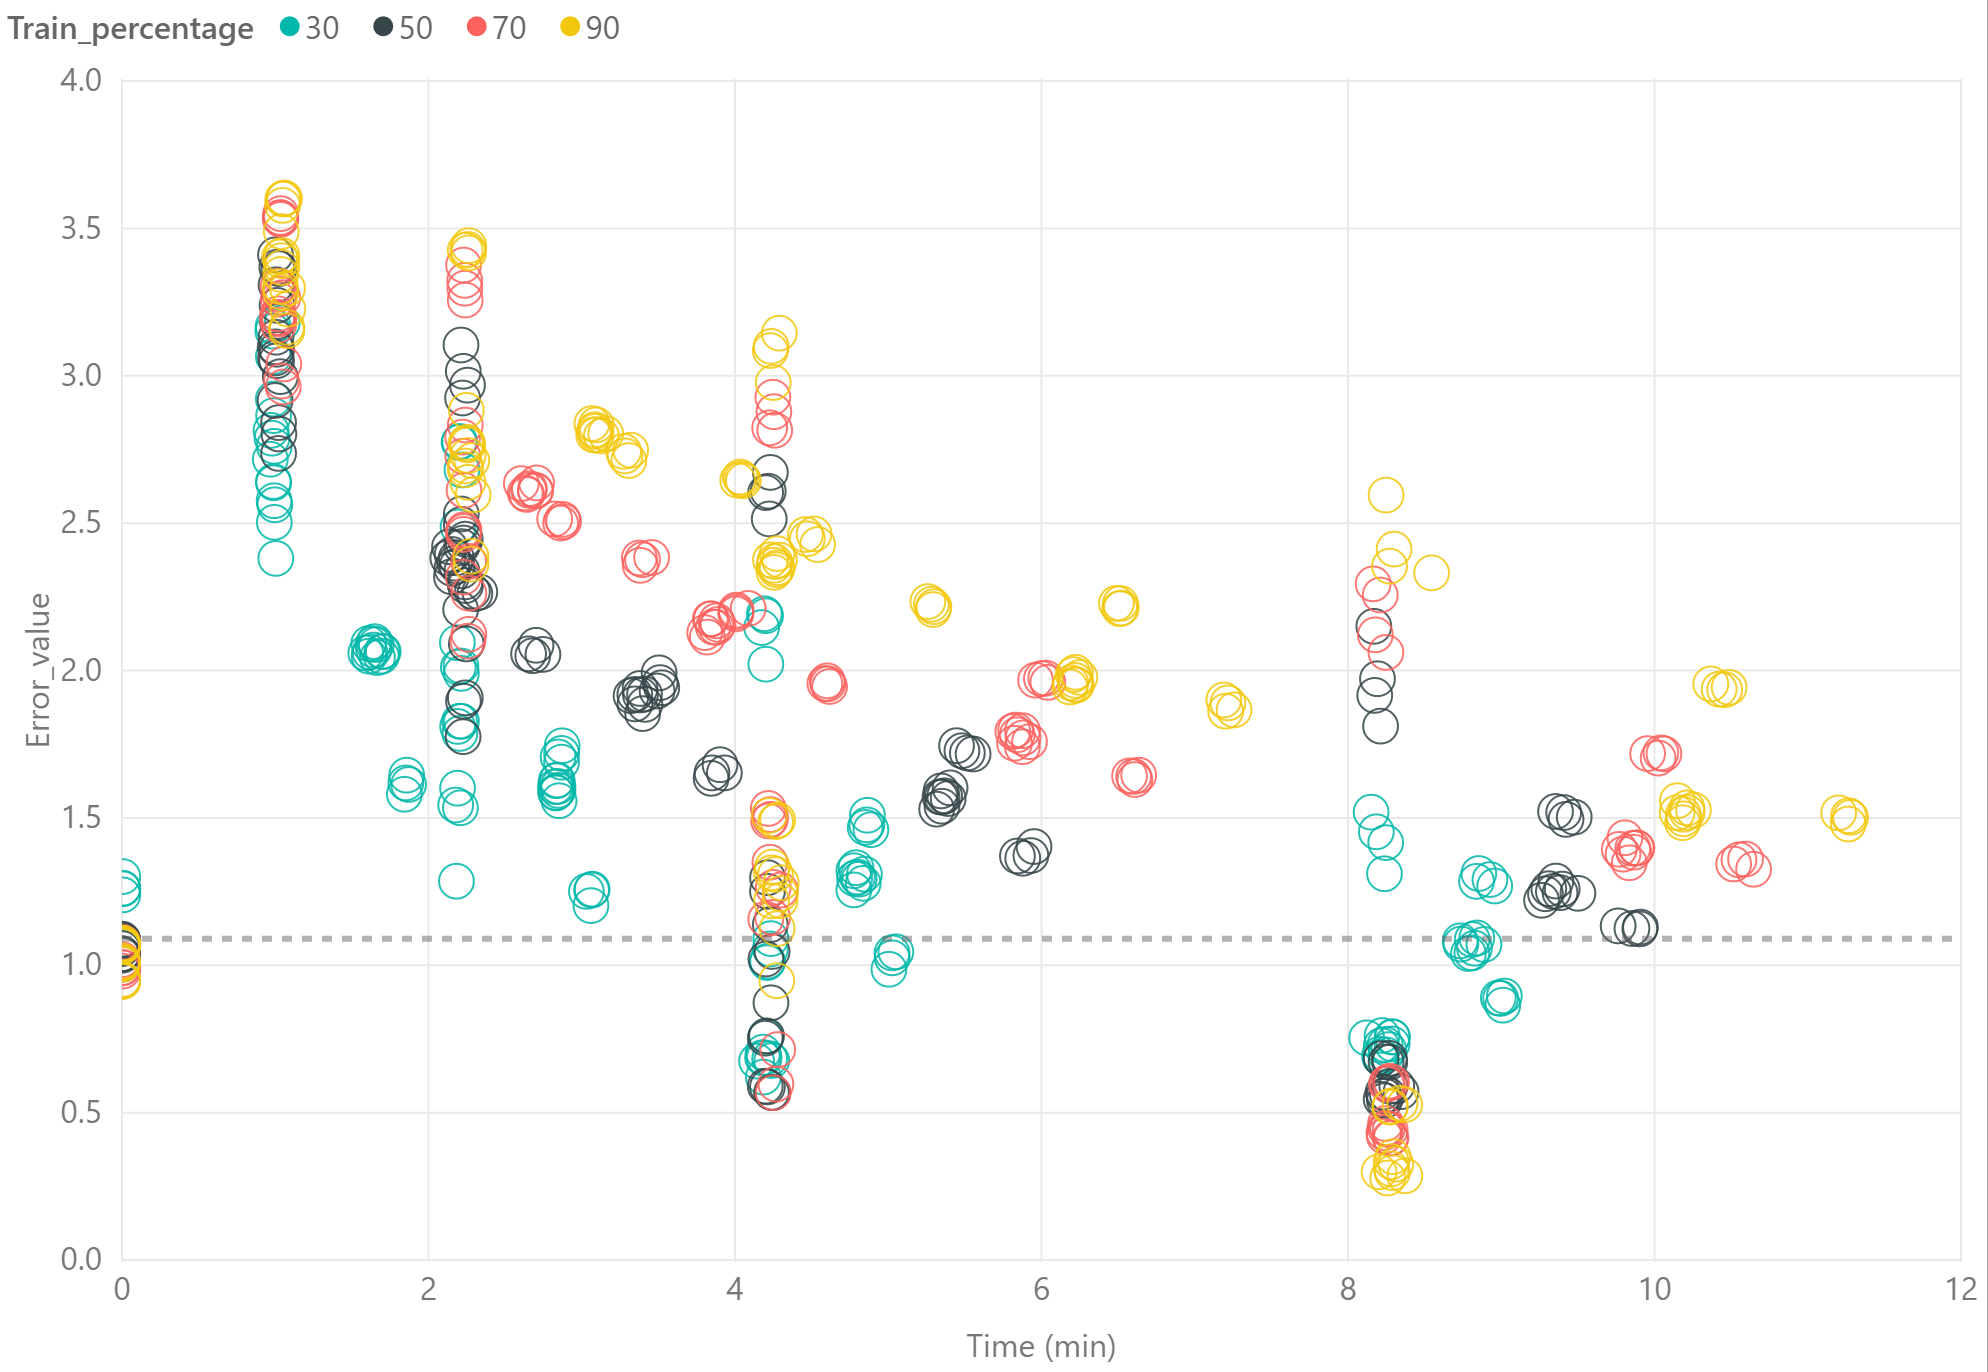
\includegraphics[width=0.60\linewidth]{../Results/Netflix/Plots/Time_RMSE_by_Train.PNG}}
%     \caption{Métodos basados en similitud: Tiempo vs RMSE}\label{fig:Time_RMSE}
% \end{figure}


\begin{figure}[htb]
    \centering

    \subfigure[Basado en usuarios, por número de vecinos]{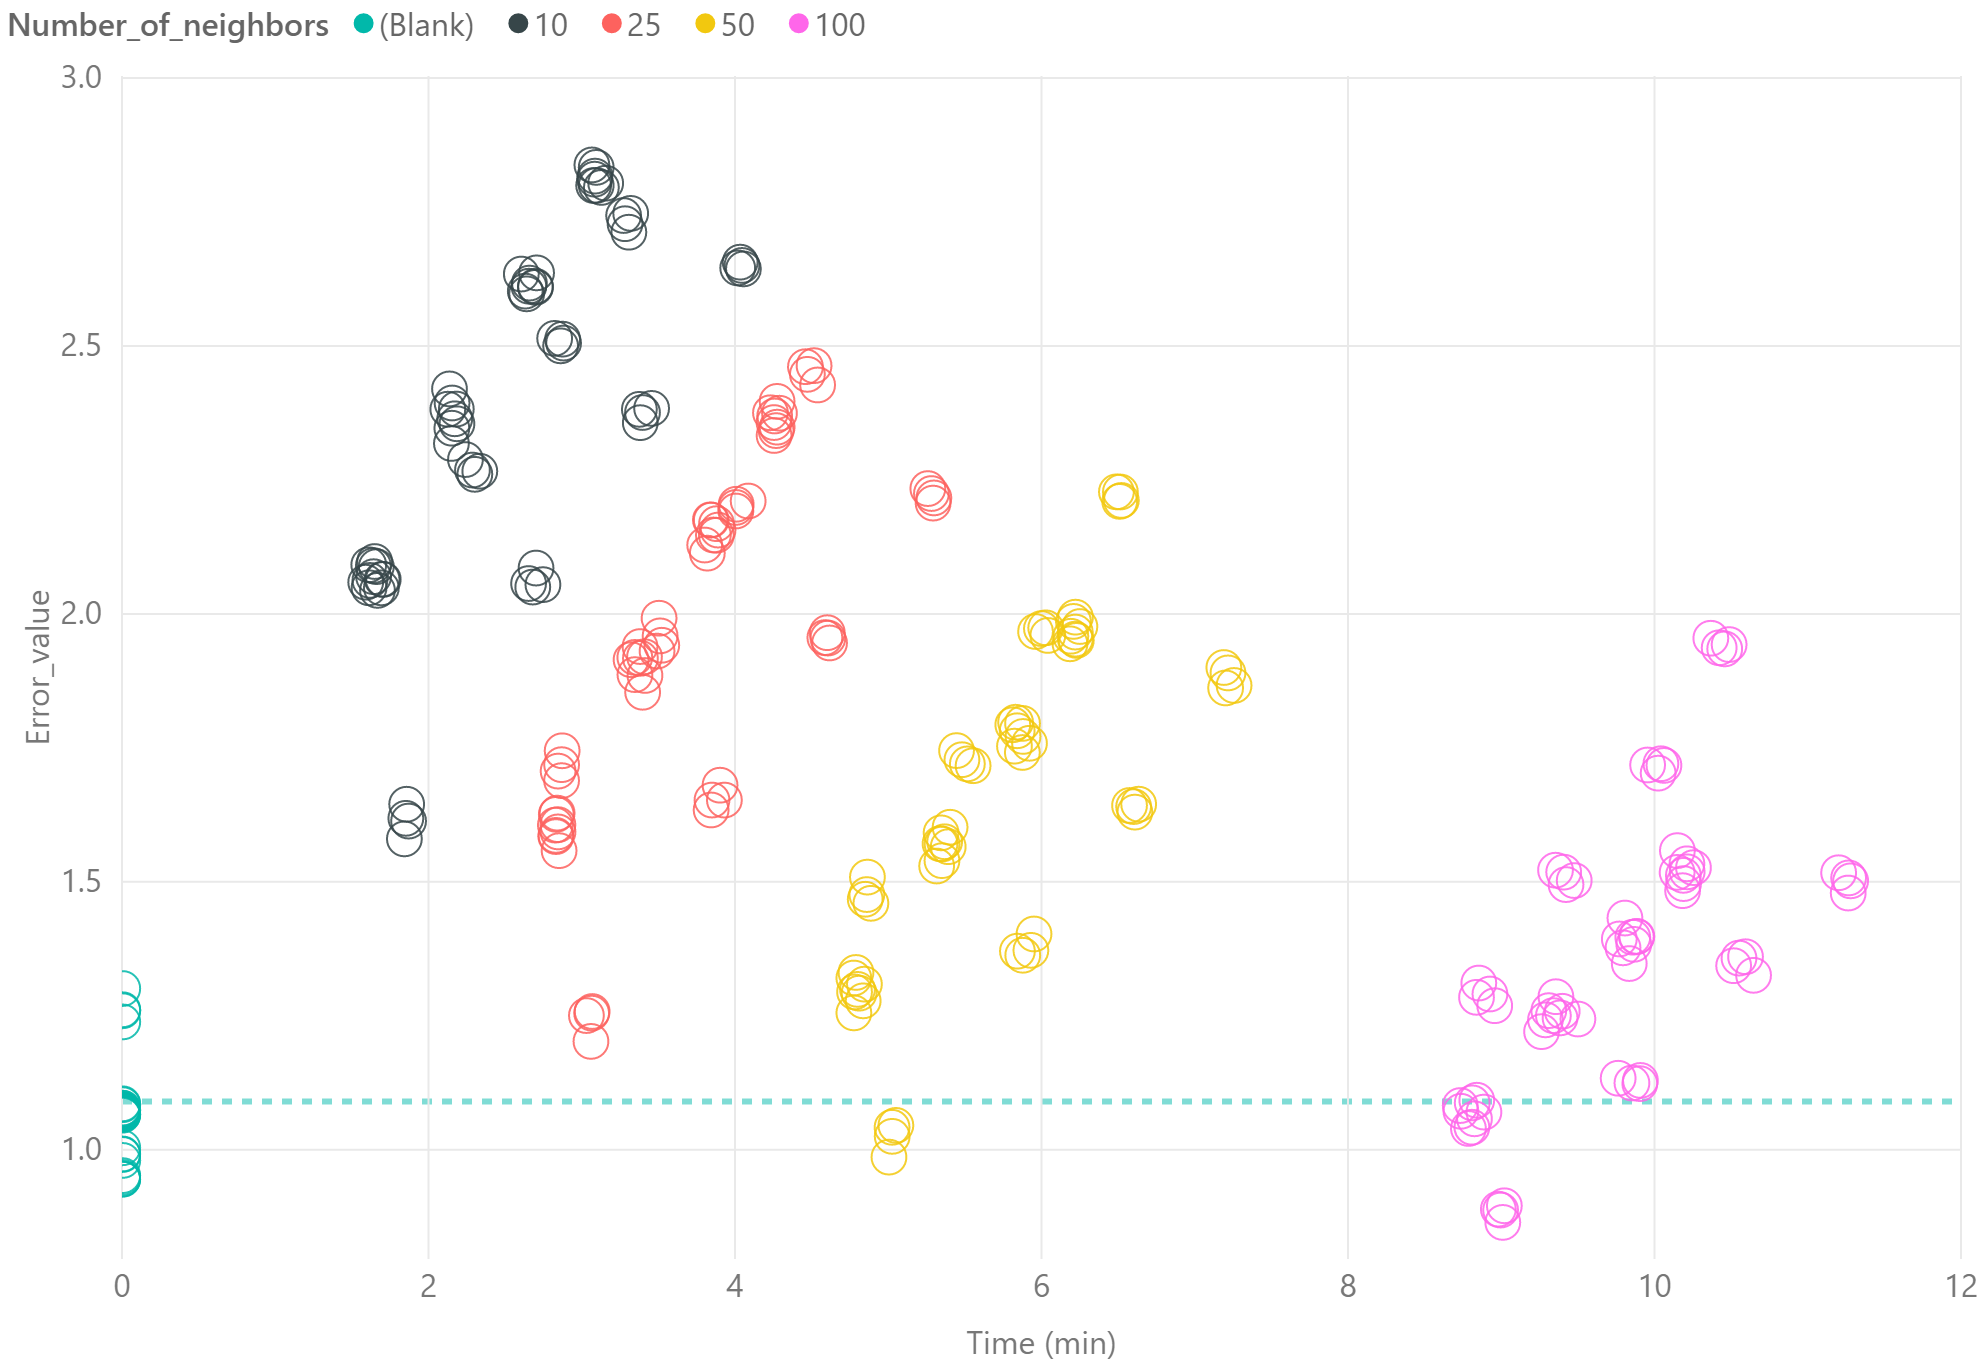
\includegraphics[width=0.48\linewidth]{../Results/Netflix/Plots/UserBased_Time_RMSE_by_Neighbors.PNG}}
    \subfigure[Basado en películas, por número de vecinos]{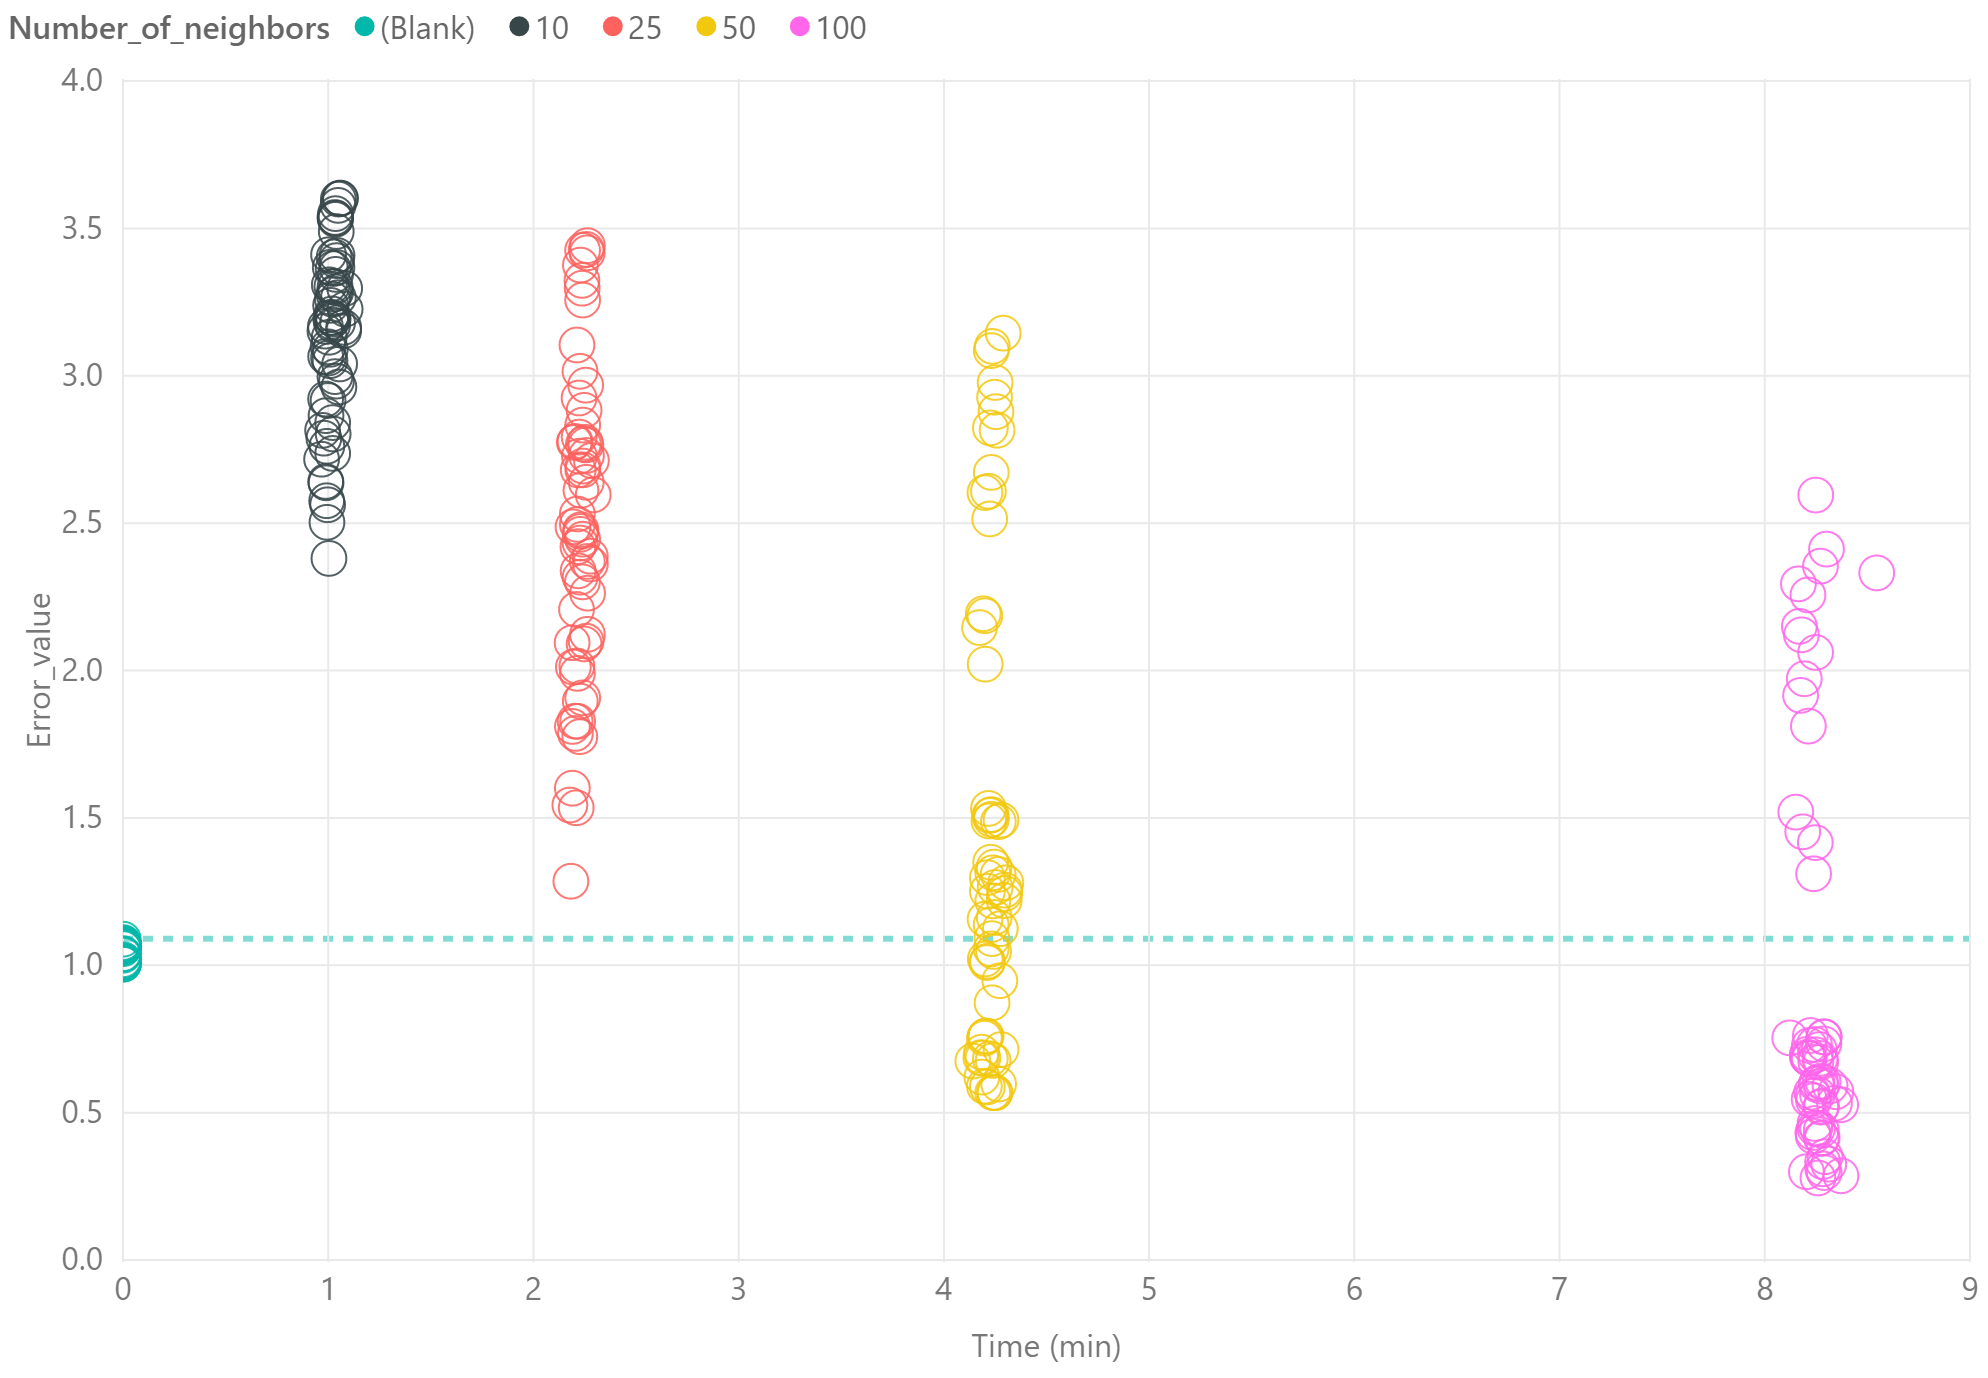
\includegraphics[width=0.48\linewidth]{../Results/Netflix/Plots/ItemBased_Time_RMSE_by_Neighbors.PNG}}

    \subfigure[Basado en usuarios, por medida de similitud]{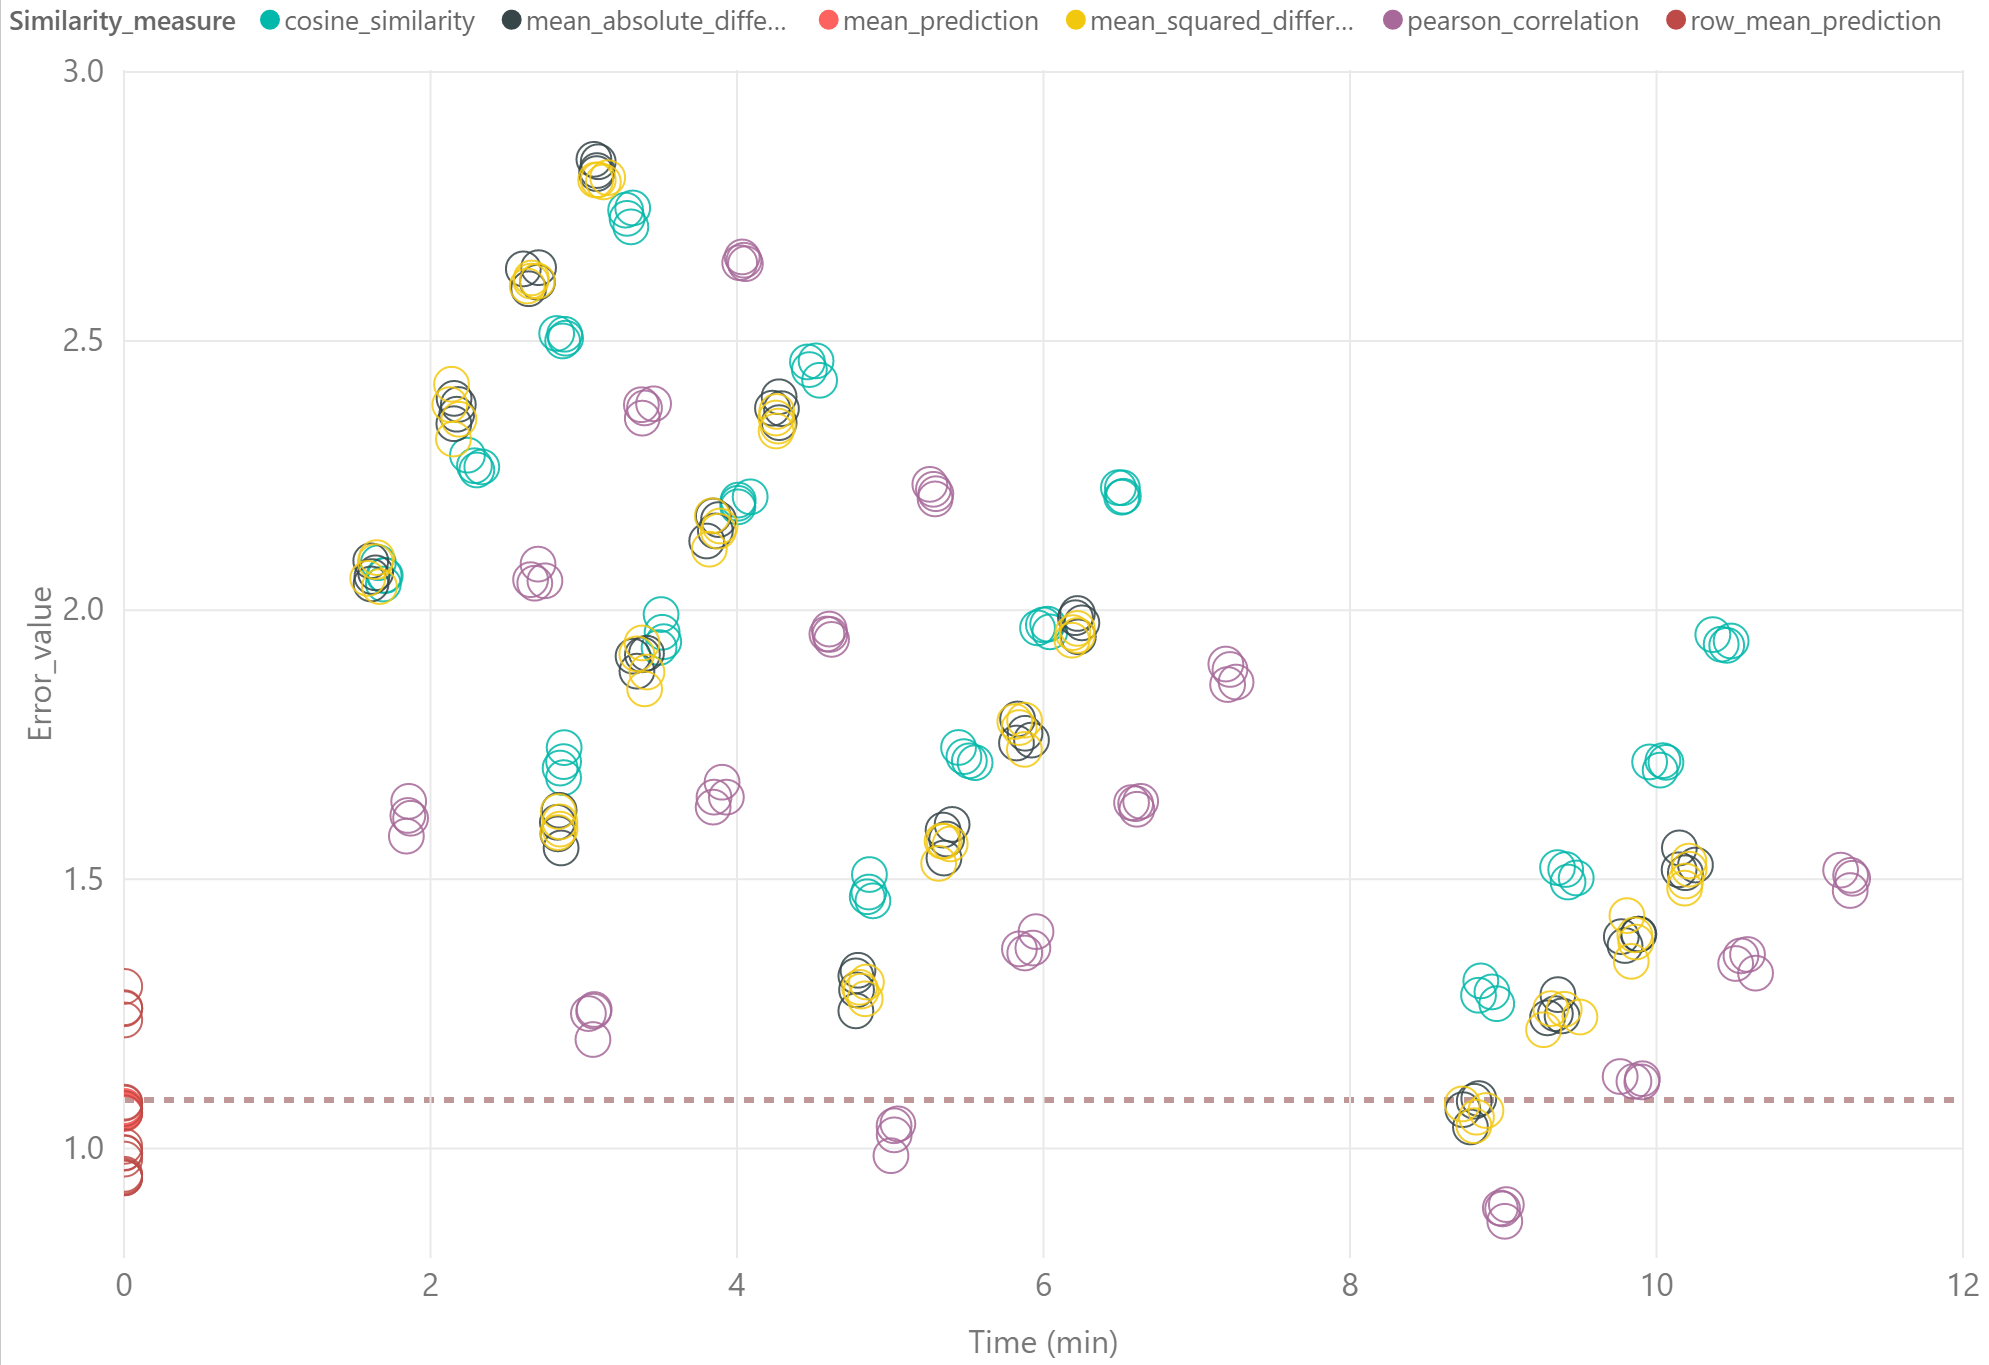
\includegraphics[width=0.48\linewidth]{../Results/Netflix/Plots/UserBased_Time_RMSE_by_Similarity.PNG}}
    \subfigure[Basado en películas, por medida de similitud]{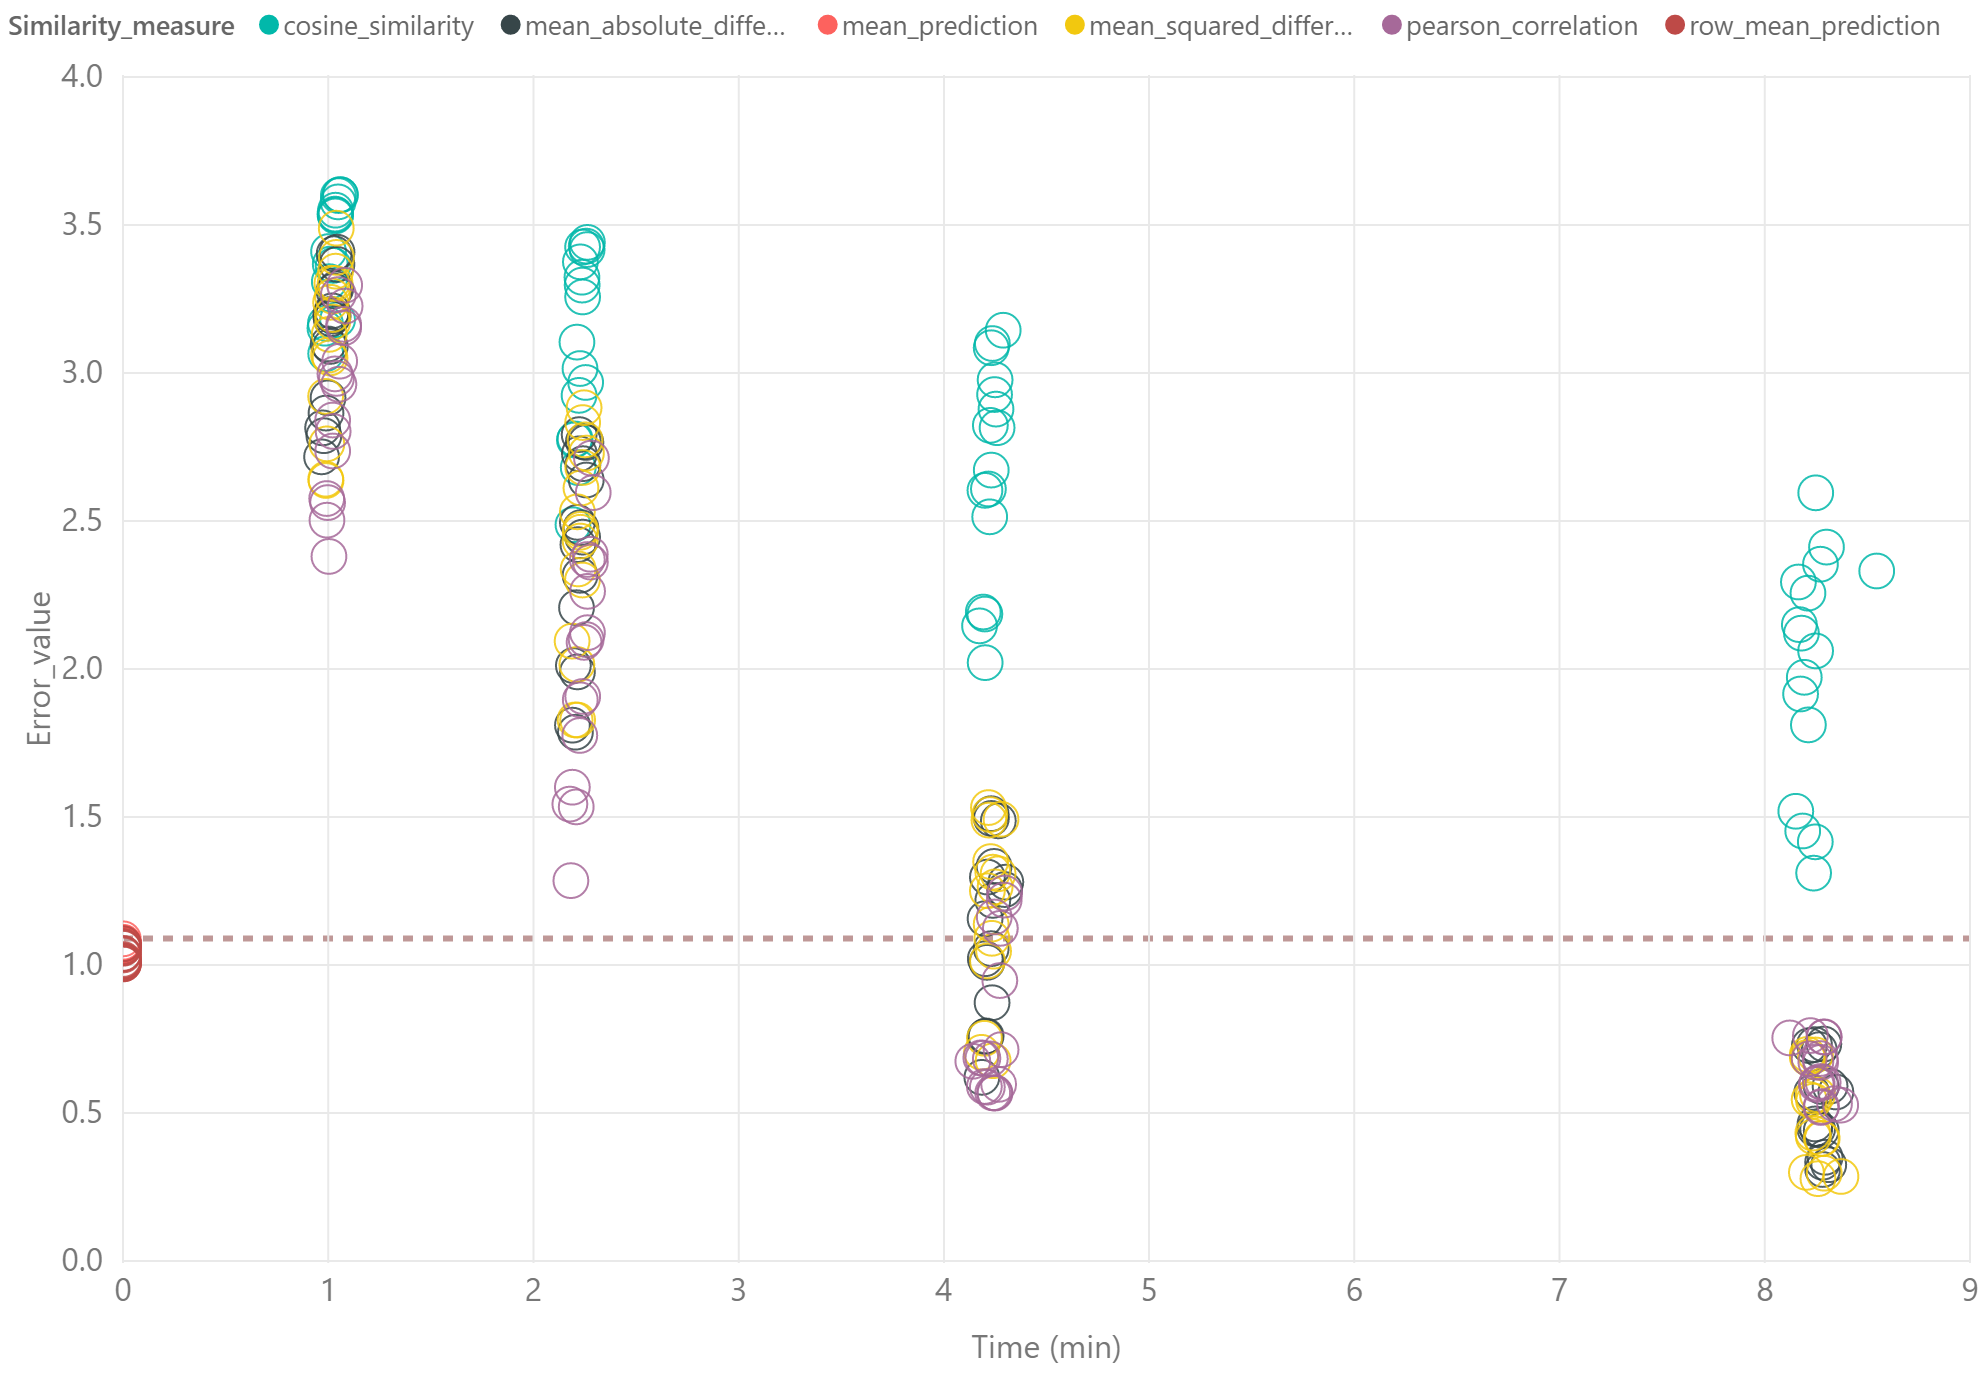
\includegraphics[width=0.48\linewidth]{../Results/Netflix/Plots/ItemBased_Time_RMSE_by_Similarity.PNG}}

    \subfigure[Basado en usuarios, por porcentaje de conjunto de entrenamiento]{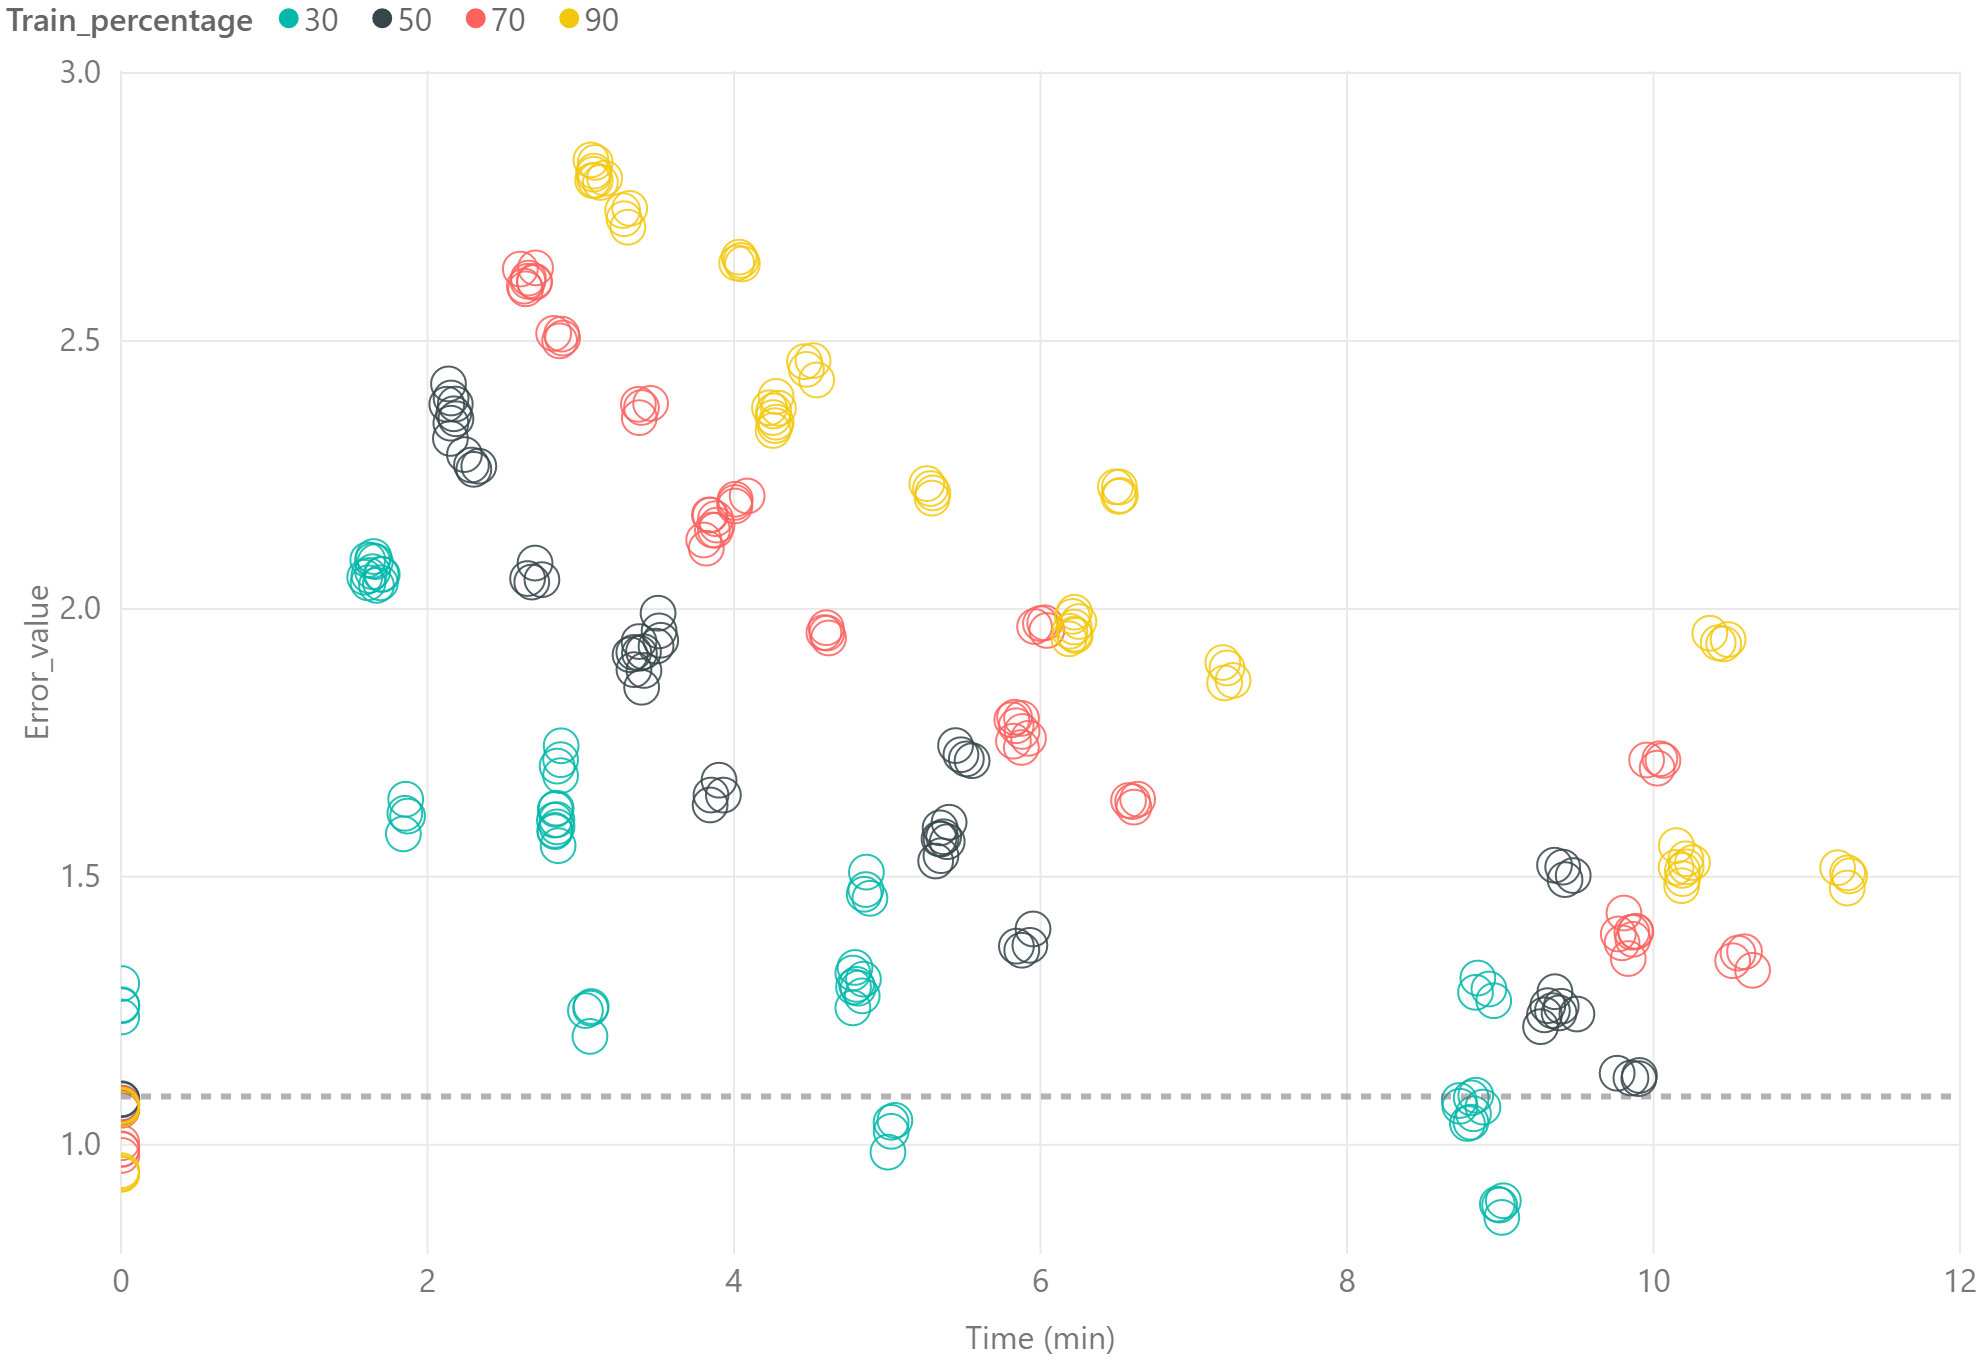
\includegraphics[width=0.48\linewidth]{../Results/Netflix/Plots/UserBased_Time_RMSE_by_Train.PNG}}
    \subfigure[Basado en películas, por porcentaje de conjunto de entrenamiento]{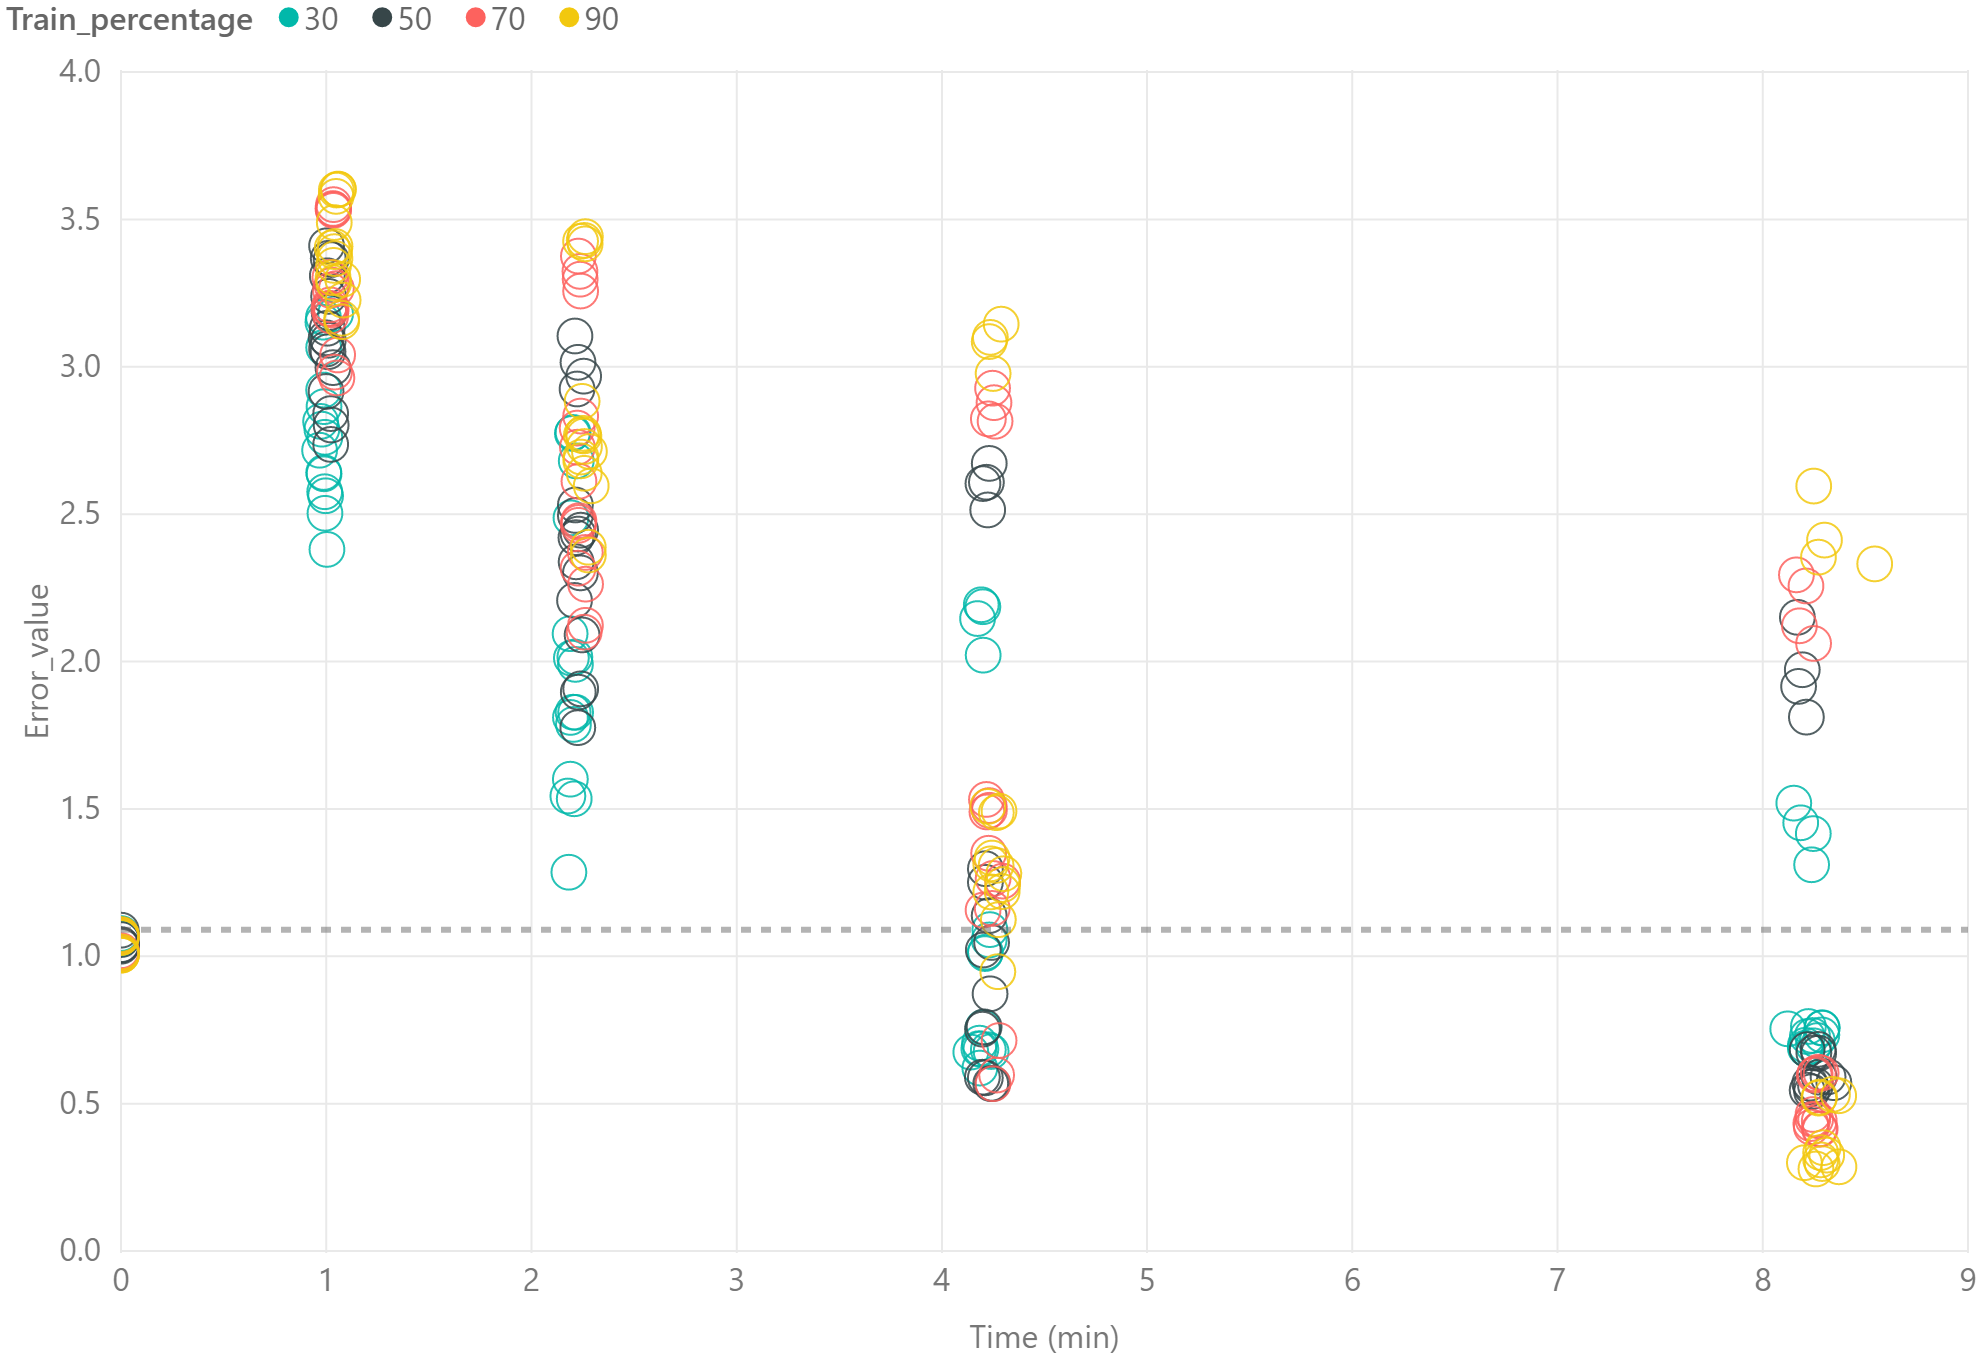
\includegraphics[width=0.48\linewidth]{../Results/Netflix/Plots/ItemBased_Time_RMSE_by_Train.PNG}}

    \caption{Métodos basados en similitud: Tiempo vs RMSE}\label{fig:resultados_similitud}
\end{figure}


\section{Medidas de evaluación}
Para evaluar cuáles han sido los mejores métodos, vamos a comparar los valores obtenidos con nuestros algoritmos contra los valores del conjunto de entrenamiento. Para esto, se pueden utilizar cualquiera de las siguientes medidas de evaluación
\begin{itemize}
    \item Root of the Mean Square Error (RMSE)
        \begin{equation}
            \RMSE = \sqrt{\frac{1}{n} \sum_{(i, j) \in \mathds{T}} (M_{i, j} - \hat M_{i, j})}
        \end{equation}
    \item Mean Absolute Error (MAE)
        \begin{equation}
            \MAE = \frac{1}{n} \sum_{(i, j) \in \mathds{T}} |M_{i, j} - \hat M_{i, j}|
        \end{equation}
\end{itemize}

Donde $\mathds{T}$ representa el conjunto de pares de índices de los valores en el conjunto de prueba.

\section{Detalles de implementación}
Los algoritmos están implementados en Python. Los resultados mostrados se obtuvieron en una computadora con las siguientes características: 8vCPUs Intel Xeon E5 v3 (2.3 GHz), 52Gb de memoria RAM y Ubuntu 14.04 LTS.

Para los métodos basados en similitud se utiliza la librería multiprocesing, que es nativa de Python, para paralelizar los cálculos de la matriz de similitud y predecir los valores utilizando las fórmulas~\ref{eq:row_based}~y~\ref{eq:col_based}.


\section{Comparación de resultados}
Utilizaremos la base de datos Netflix3m1k para hacer las pruebas de los algoritmos.

Comenzaremos comparando los métodos basados en similitud de filas o columnas. Para esto, se hicieron pruebas cambiando los siguientes parámetros:
\begin{itemize}
    \item Número de vecinos: $\{10, 25, 50, 100\}$
    \item Porcentaje del conjunto de entrenamiento: $\{30, 50, 70, 90\}$.
    \item Porcentaje del conjunto de prueba: $\{10, 20, 30, 50\}$.
    \item Medida de similitud: Se utilizaron todas las de la sección~\ref{sec:medidas_similitud}.
\end{itemize}
En la figura~\ref{fig:resultados_similitud} se muestran los resultados obtenidos. Las imágenes de la primera columna corresponden a los resultados obtenidos midiendo la similitud por filas (correspondientes a usuarios) y la segunda columna son los resultados obtenidos midiendo la similitud por columnas (correspondientes a películas). Cada una de las gráficas muestra el tiempo de ejecución en el eje $X$ y el error $\RMSE$ en el eje $Y$.

Algunas de las conclusiones que podemos obtener de estas gráficas son las siguientes:
\begin{itemize}
    \item Los tiempos de ejecución dependen mucho más fuerte del número de vecinos que del porcentaje del conjunto de entrenamiento.
    \item Para esta base de datos, se obtienen mejores resultados si utilizamos métodos basados en columnas.
    \item La peor medida de similitud es la de coseno y las mejores son mean square difference y correlación de Pearson.

        La línea punteada horizontal en las gráficas corresponde al valor del $\RMSE$ que se obtiene en promedio utilizando los métodos basados en promedios de la sección~\ref{sec:basados_en_promedios}. Notemos que únicamente a partir de utilizar 50 vecinos empezamos a tener resultados que mejoran este valor, sin embargo las mejoras son bastante significativas.
\end{itemize}

\end{document}
